\section{Índices espectrales}
\subsection{Análisis espectral}

\begin{frame}{\secname : \subsecname}
  \begin{figure}
    \centering
    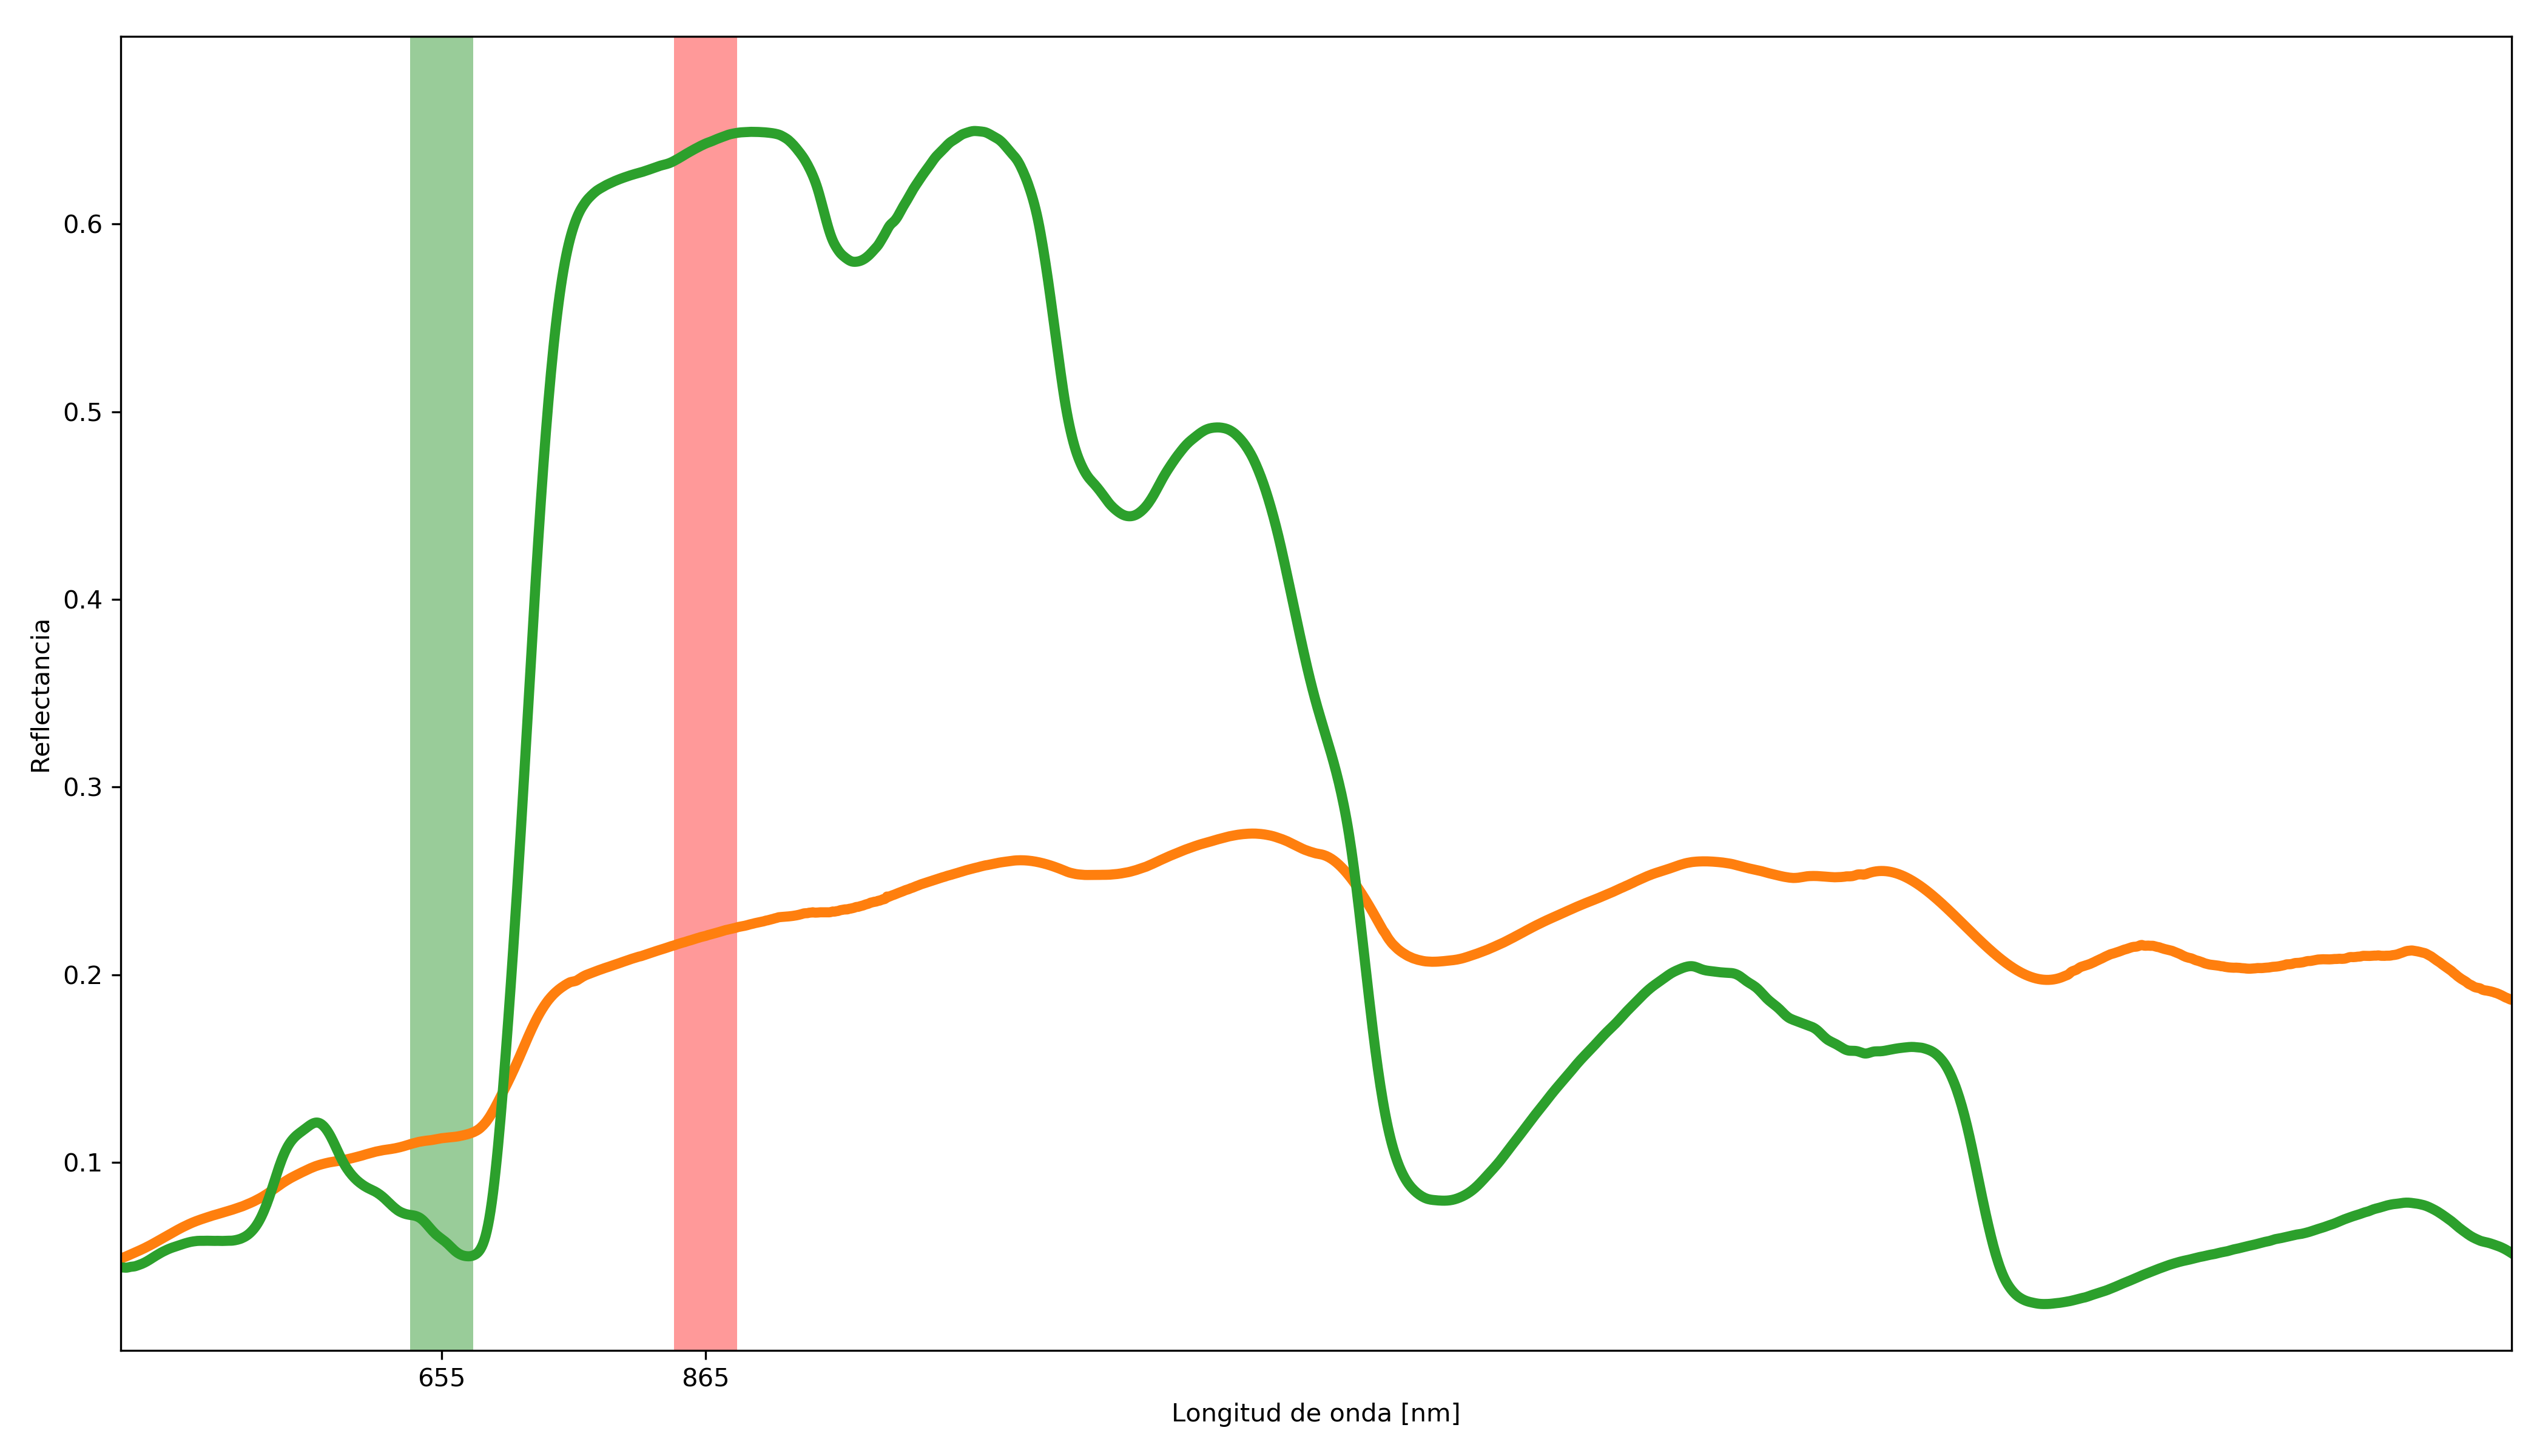
\includegraphics[width=0.8\textwidth]{fig:firmasin.png}
    \caption{Firma espectral del suelo y de la vegetación.}
    \label{}
  \end{figure}
\end{frame}
%--- Next Frame ---%

\begin{frame}{\secname : \subsecname}
  \begin{figure}
    \centering
    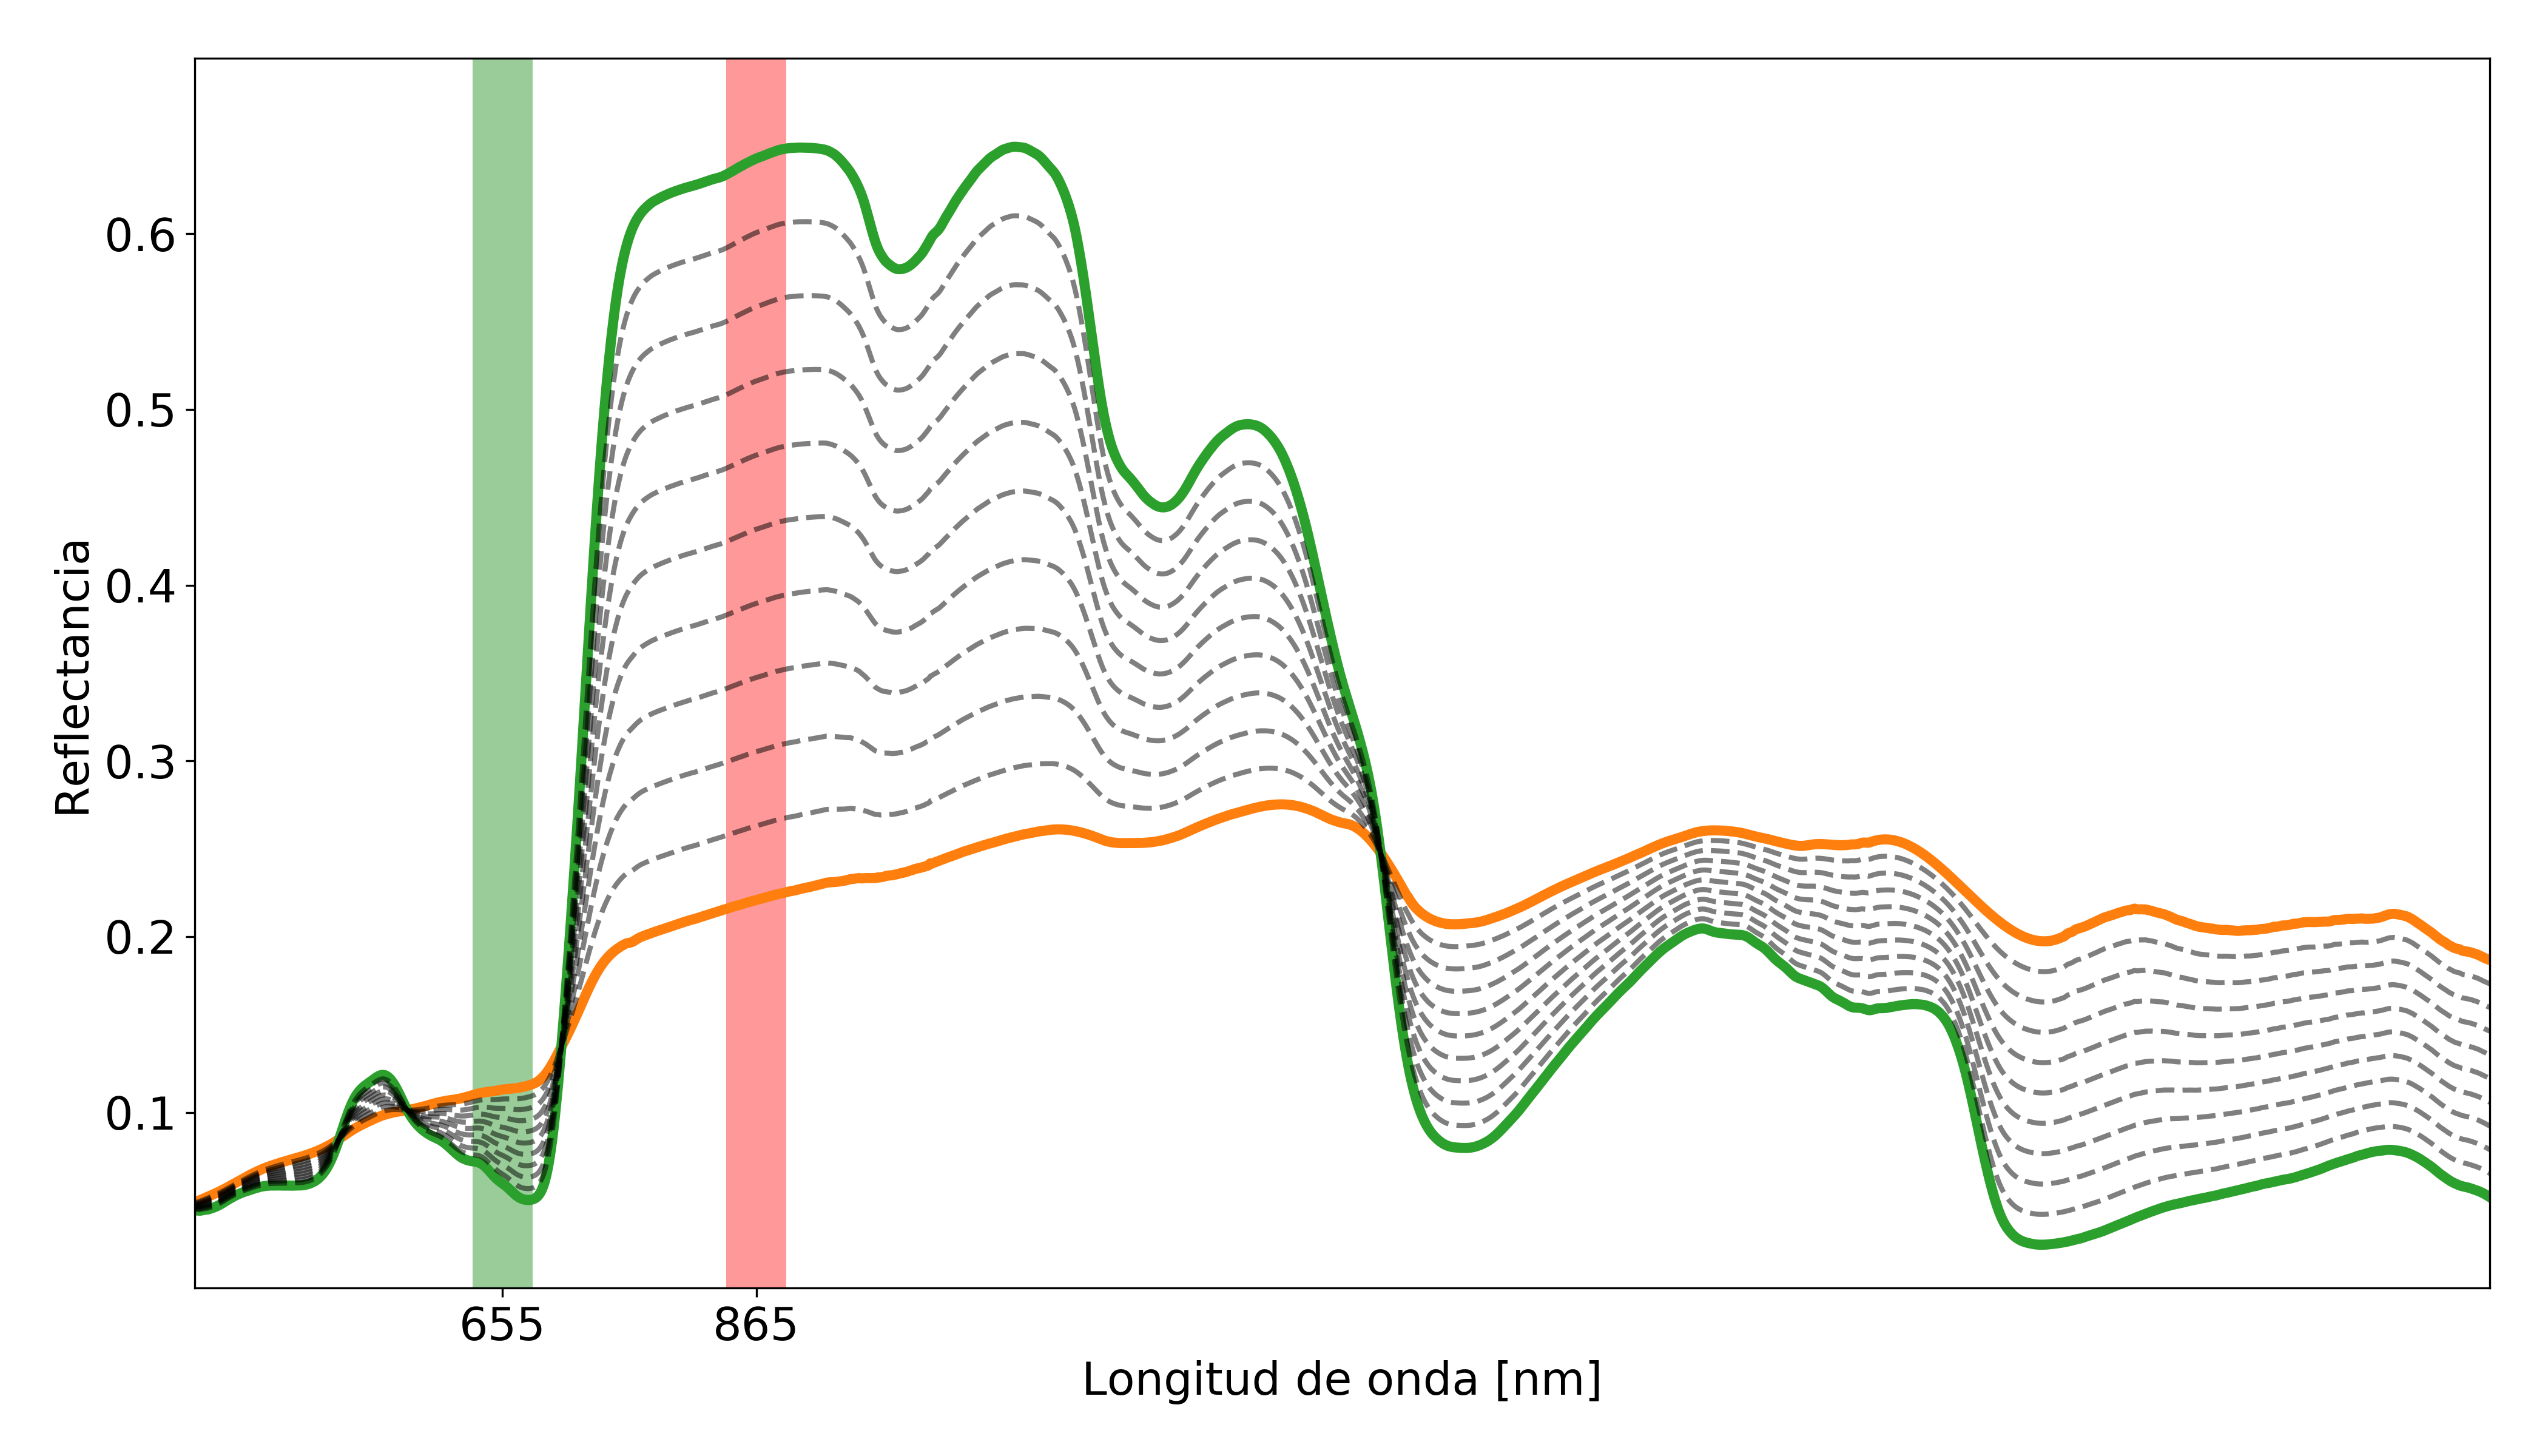
\includegraphics[width=0.8\textwidth]{fig:firmavar.png}
    \caption{Variacion de la firam espectral según porcentaje de cobertura de vegetación.}
    \label{}
  \end{figure}
\end{frame}
%--- Next Frame ---%

\subsection{Índices espectrales}

\begin{frame}{\secname : \subsecname}
  \begin{figure}
    \centering
    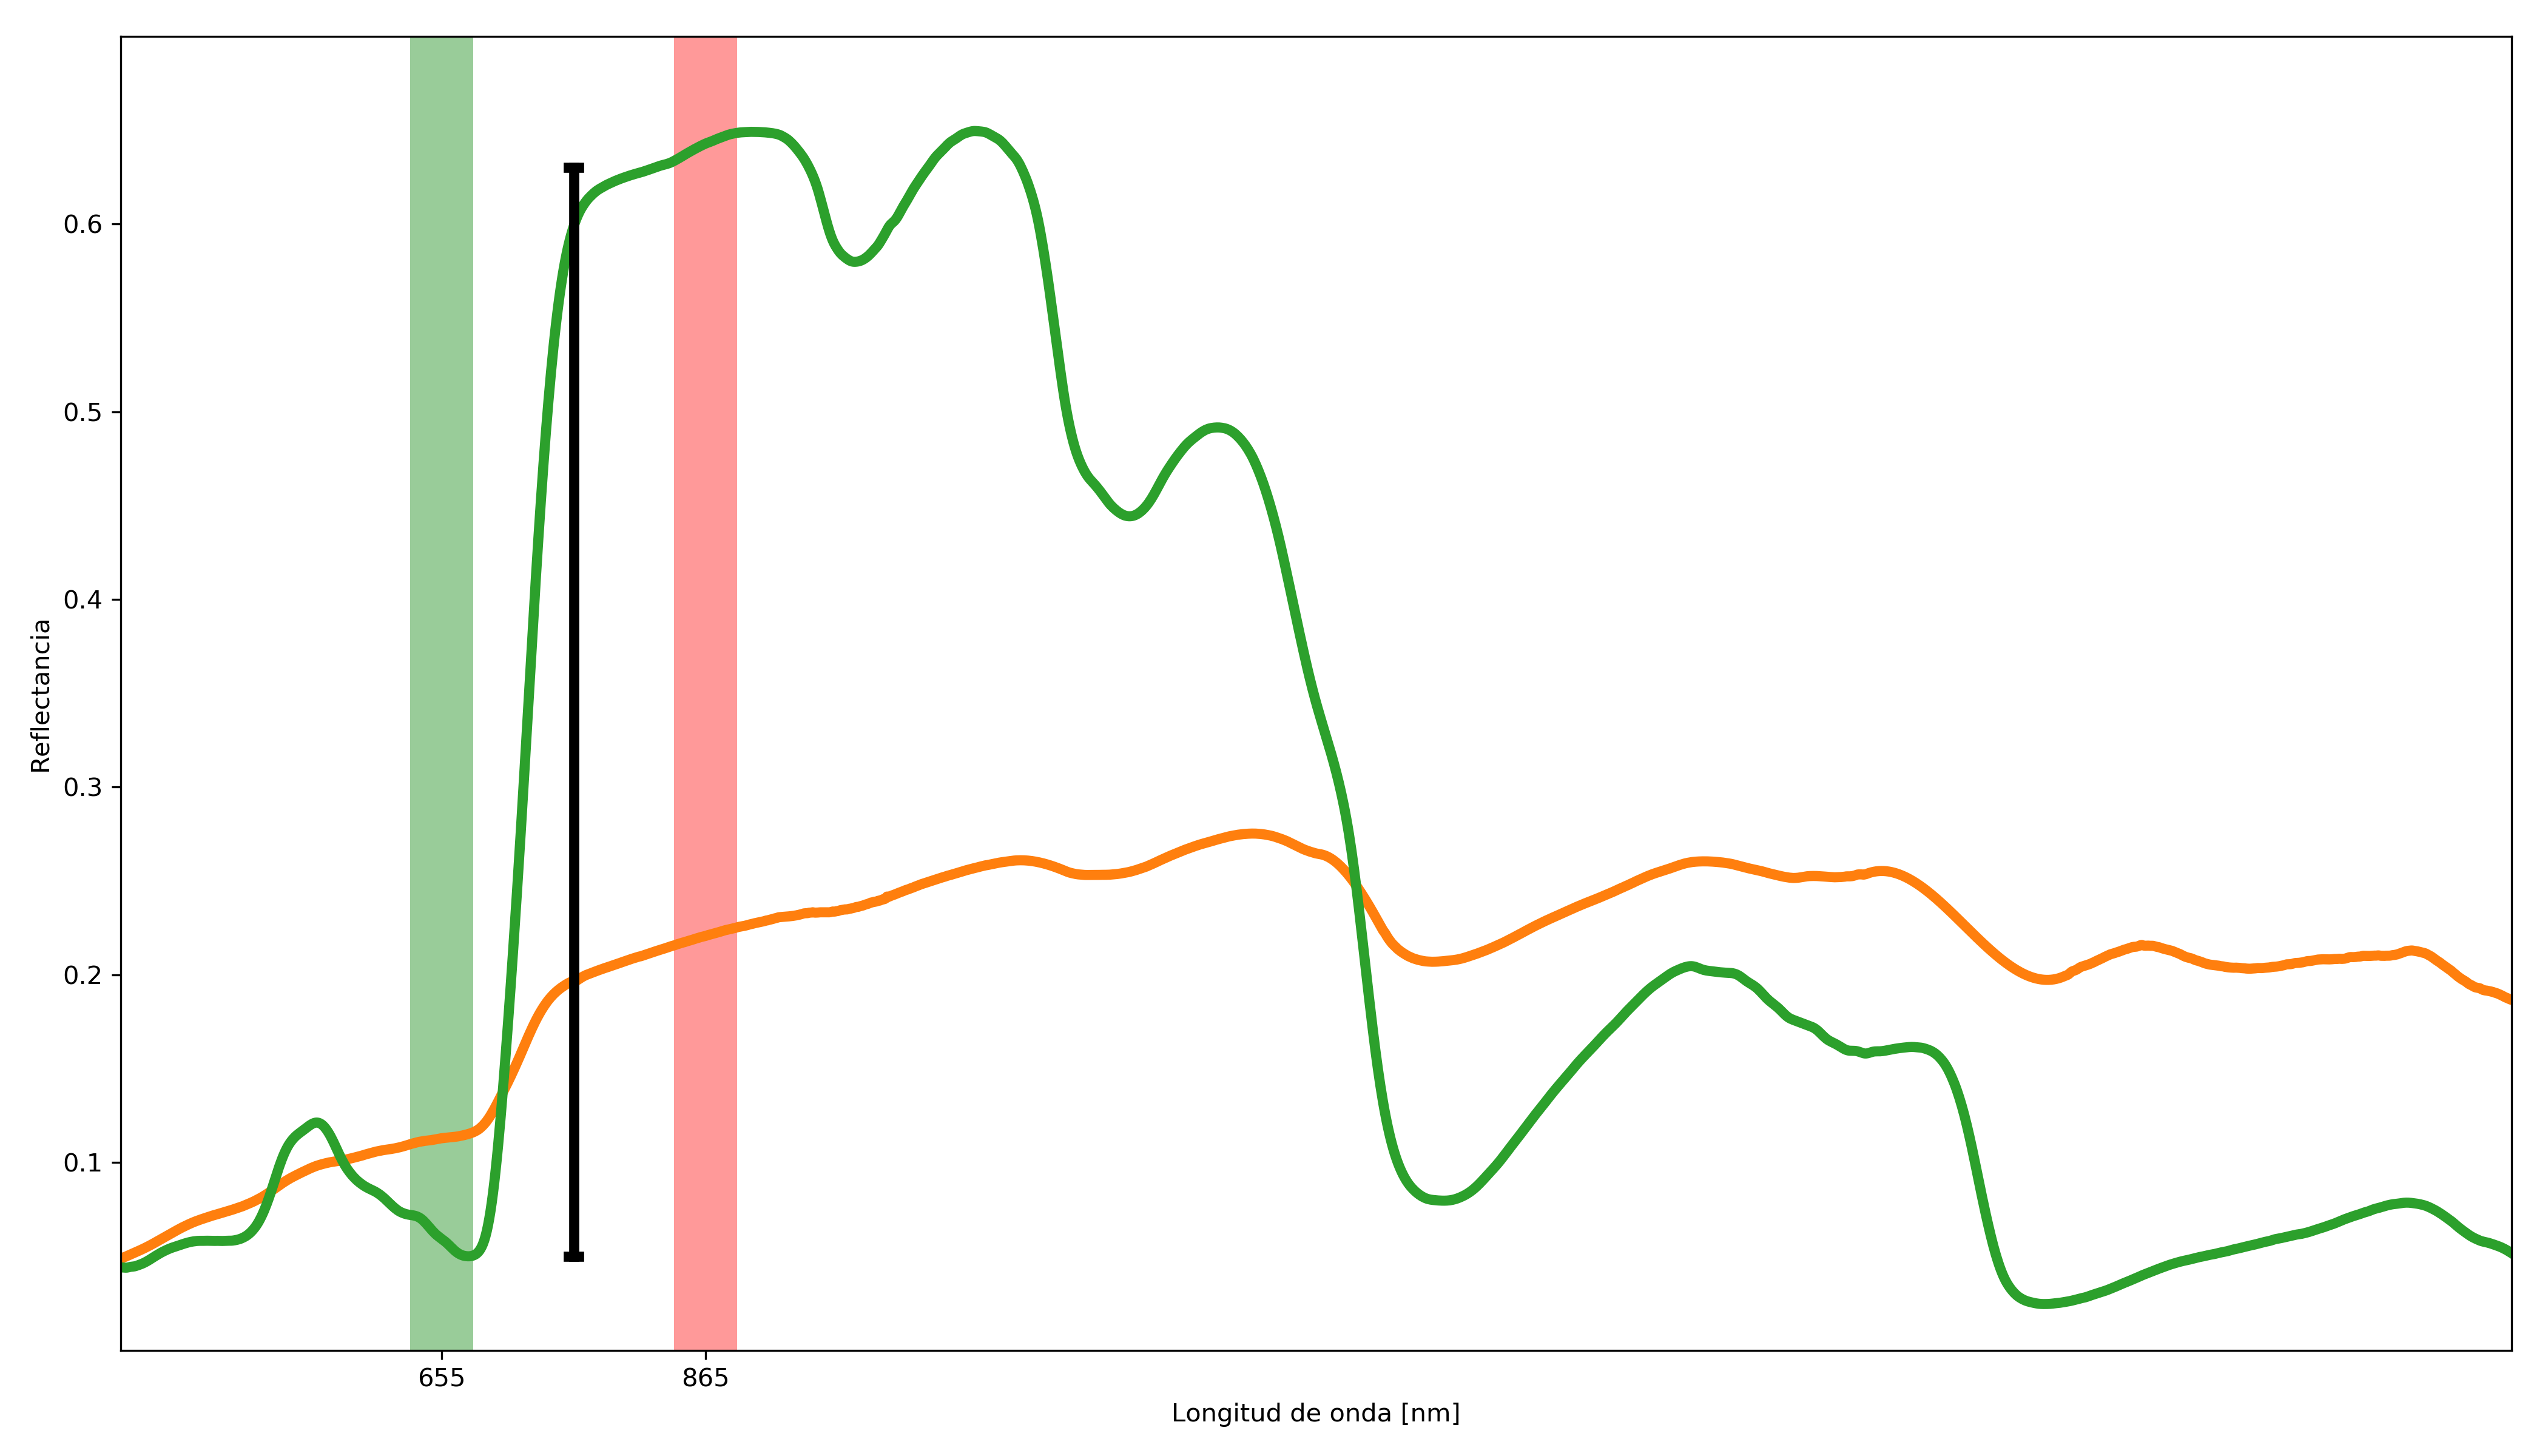
\includegraphics[width=0.8\textwidth]{fig:firmasalto.png}
    \caption{Salto $\rho_{nir}$ - $\rho_{red}$}
    \label{}
  \end{figure}
\end{frame}

%--- Next Frame ---%

\begin{frame}{\secname : \subsecname}
\begin{block}{Normalized Difference Vegetation Index - NDVI}
  Definimos al NDVI como
  \begin{equation}
    NDVI = \frac{\rho_{nir}-\rho_{red}}{\rho_{nir}+\rho_{red}}
  \end{equation}
  con $\rho_{nir}$, $\rho_{red}$ las reflectancias en el infrarrojo cercano y el rojo.
\end{block}
\begin{block}{Observación}
    \begin{itemize}[<+->]
        \item La reflectancia del suelo lo puede afectar.
        \item Satura cuando el canopeo es muy denso.
    \end{itemize}
\end{block}
\end{frame}
%--- Next Frame ---%

\begin{frame}{\secname : \subsecname}
  \begin{figure}
    \centering
    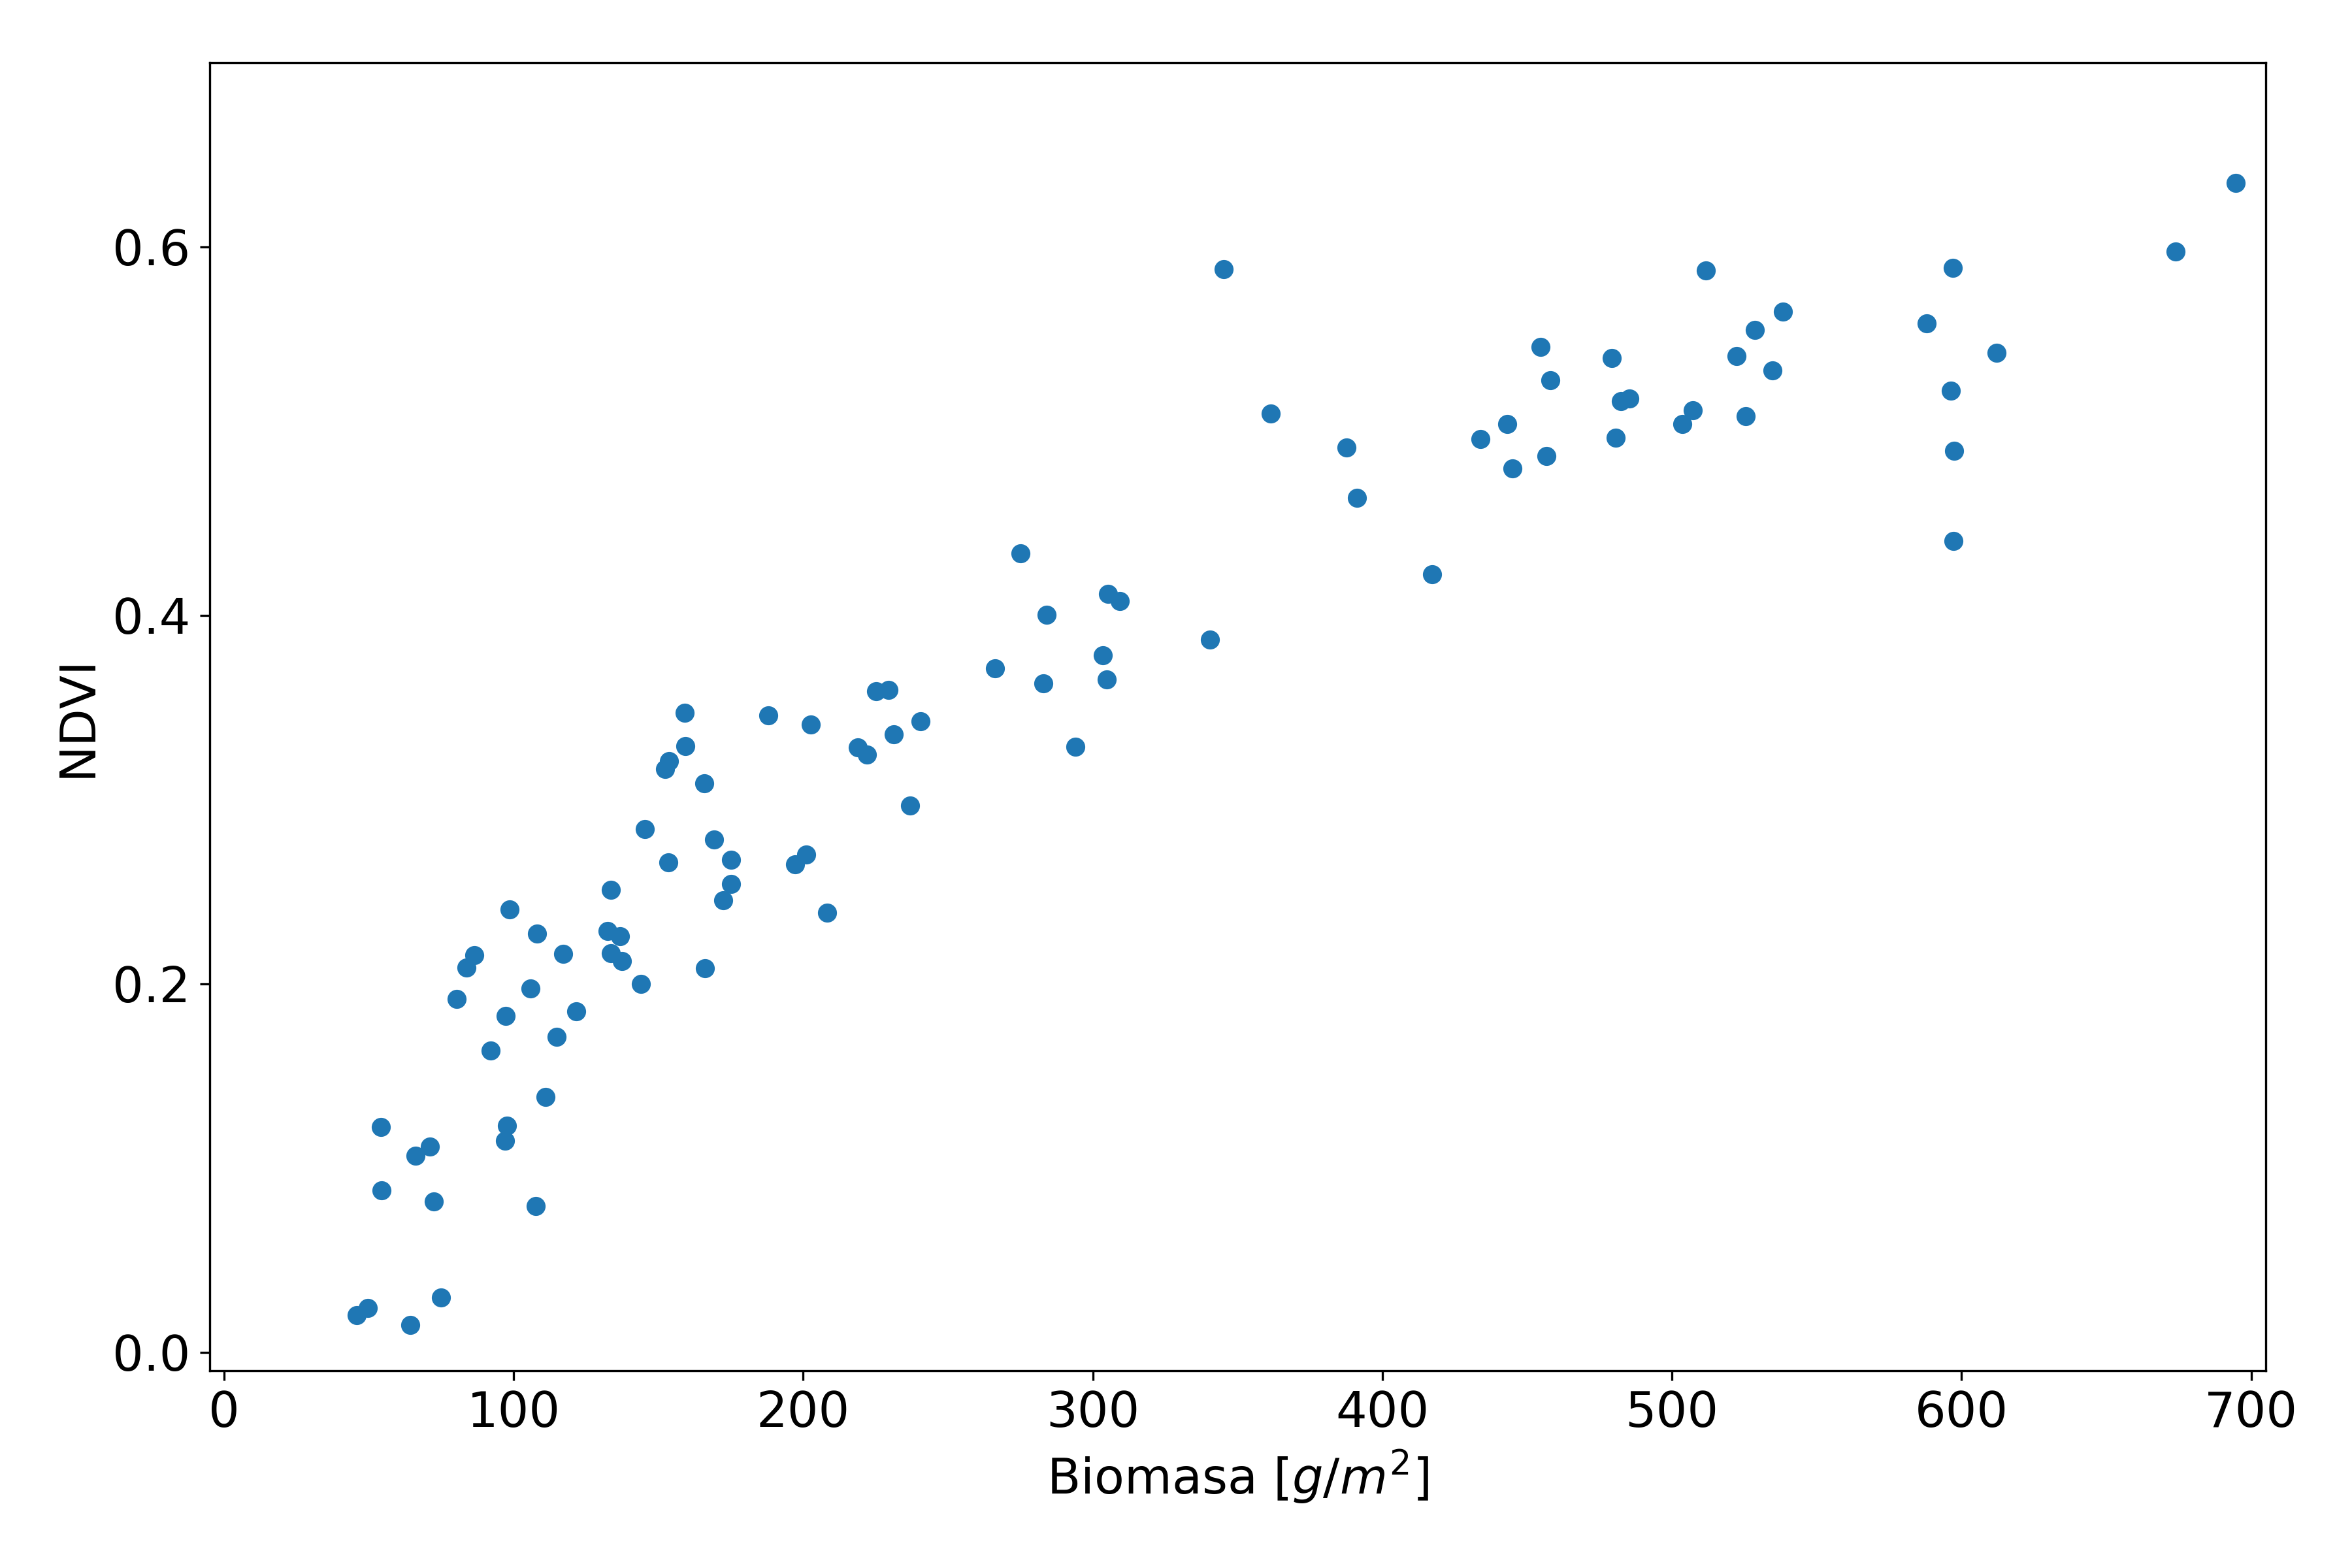
\includegraphics[width=0.7\textwidth]{fig:biomasa.png}
    \caption{Relación entre la biomasa y el NDVI.}
    \label{}
  \end{figure}
\end{frame}
%--- Next Frame ---%

\begin{frame}{\secname : \subsecname}
    \begin{block}{Soil Adjusted Vegetation Index - SAVI}
        \begin{equation}
            SAVI = \frac{\rho_n-\rho_r}{\rho_n+\rho_r+L}(1+L)
        \end{equation}
    \end{block}\pause\
    \begin{block}{Observación}
        \begin{itemize}[<+->]
            \item Suele ajustar mejor a las variaciones de reflectancia del
                suelo.
            \item Es difícil conocer el valor de $L$ a priori. \begin{equation}
        L=0.5
    \end{equation}
        \end{itemize}
    \end{block}
\end{frame}

\begin{frame}{\secname : \subsecname}
    \begin{block}{Enhanced Vegetation Index - EVI}
        \begin{equation}
            EVI = G\frac{\rho_n - \rho_r}{\rho_n+C_1\rho_r-C_2\rho_b+L}(1+L)
        \end{equation}
    \end{block}
    donde
    \begin{itemize}
        \item $G  \sim 2.5$
        \item $C1 \sim 6.0$
        \item $C2 \sim 7.5$
        \item $L  \sim 1.0$
    \end{itemize}
\end{frame}

\begin{frame}{\secname : \subsecname}
Muchas gracias.
\end{frame}
%--- Next Frame ---%
